\documentclass[1p]{elsarticle_modified}
%\bibliographystyle{elsarticle-num}

%\usepackage[colorlinks]{hyperref}
%\usepackage{abbrmath_seonhwa} %\Abb, \Ascr, \Acal ,\Abf, \Afrak
\usepackage{amsfonts}
\usepackage{amssymb}
\usepackage{amsmath}
\usepackage{amsthm}
\usepackage{scalefnt}
\usepackage{amsbsy}
\usepackage{kotex}
\usepackage{caption}
\usepackage{subfig}
\usepackage{color}
\usepackage{graphicx}
\usepackage{xcolor} %% white, black, red, green, blue, cyan, magenta, yellow
\usepackage{float}
\usepackage{setspace}
\usepackage{hyperref}

\usepackage{tikz}
\usetikzlibrary{arrows}

\usepackage{multirow}
\usepackage{array} % fixed length table
\usepackage{hhline}

%%%%%%%%%%%%%%%%%%%%%
\makeatletter
\renewcommand*\env@matrix[1][\arraystretch]{%
	\edef\arraystretch{#1}%
	\hskip -\arraycolsep
	\let\@ifnextchar\new@ifnextchar
	\array{*\c@MaxMatrixCols c}}
\makeatother %https://tex.stackexchange.com/questions/14071/how-can-i-increase-the-line-spacing-in-a-matrix
%%%%%%%%%%%%%%%

\usepackage[normalem]{ulem}

\newcommand{\msout}[1]{\ifmmode\text{\sout{\ensuremath{#1}}}\else\sout{#1}\fi}
%SOURCE: \msout is \stkout macro in https://tex.stackexchange.com/questions/20609/strikeout-in-math-mode

\newcommand{\cancel}[1]{
	\ifmmode
	{\color{red}\msout{#1}}
	\else
	{\color{red}\sout{#1}}
	\fi
}

\newcommand{\add}[1]{
	{\color{blue}\uwave{#1}}
}

\newcommand{\replace}[2]{
	\ifmmode
	{\color{red}\msout{#1}}{\color{blue}\uwave{#2}}
	\else
	{\color{red}\sout{#1}}{\color{blue}\uwave{#2}}
	\fi
}

\newcommand{\Sol}{\mathcal{S}} %segment
\newcommand{\D}{D} %diagram
\newcommand{\A}{\mathcal{A}} %arc


%%%%%%%%%%%%%%%%%%%%%%%%%%%%%5 test

\def\sl{\operatorname{\textup{SL}}(2,\Cbb)}
\def\psl{\operatorname{\textup{PSL}}(2,\Cbb)}
\def\quan{\mkern 1mu \triangleright \mkern 1mu}

\theoremstyle{definition}
\newtheorem{thm}{Theorem}[section]
\newtheorem{prop}[thm]{Proposition}
\newtheorem{lem}[thm]{Lemma}
\newtheorem{ques}[thm]{Question}
\newtheorem{cor}[thm]{Corollary}
\newtheorem{defn}[thm]{Definition}
\newtheorem{exam}[thm]{Example}
\newtheorem{rmk}[thm]{Remark}
\newtheorem{alg}[thm]{Algorithm}

\newcommand{\I}{\sqrt{-1}}
\begin{document}

%\begin{frontmatter}
%
%\title{Boundary parabolic representations of knots up to 8 crossings}
%
%%% Group authors per affiliation:
%\author{Yunhi Cho} 
%\address{Department of Mathematics, University of Seoul, Seoul, Korea}
%\ead{yhcho@uos.ac.kr}
%
%
%\author{Seonhwa Kim} %\fnref{s_kim}}
%\address{Center for Geometry and Physics, Institute for Basic Science, Pohang, 37673, Korea}
%\ead{ryeona17@ibs.re.kr}
%
%\author{Hyuk Kim}
%\address{Department of Mathematical Sciences, Seoul National University, Seoul 08826, Korea}
%\ead{hyukkim@snu.ac.kr}
%
%\author{Seokbeom Yoon}
%\address{Department of Mathematical Sciences, Seoul National University, Seoul, 08826,  Korea}
%\ead{sbyoon15@snu.ac.kr}
%
%\begin{abstract}
%We find all boundary parabolic representation of knots up to 8 crossings.
%
%\end{abstract}
%\begin{keyword}
%    \MSC[2010] 57M25 
%\end{keyword}
%
%\end{frontmatter}

%\linenumbers
%\tableofcontents
%
\newcommand\colored[1]{\textcolor{white}{\rule[-0.35ex]{0.8em}{1.4ex}}\kern-0.8em\color{red} #1}%
%\newcommand\colored[1]{\textcolor{white}{ #1}\kern-2.17ex	\textcolor{white}{ #1}\kern-1.81ex	\textcolor{white}{ #1}\kern-2.15ex\color{red}#1	}

{\Large $\underline{12n_{0331}~(K12n_{0331})}$}

\setlength{\tabcolsep}{10pt}
\renewcommand{\arraystretch}{1.6}
\vspace{1cm}\begin{tabular}{m{100pt}>{\centering\arraybackslash}m{274pt}}
\multirow{5}{120pt}{
	\centering
	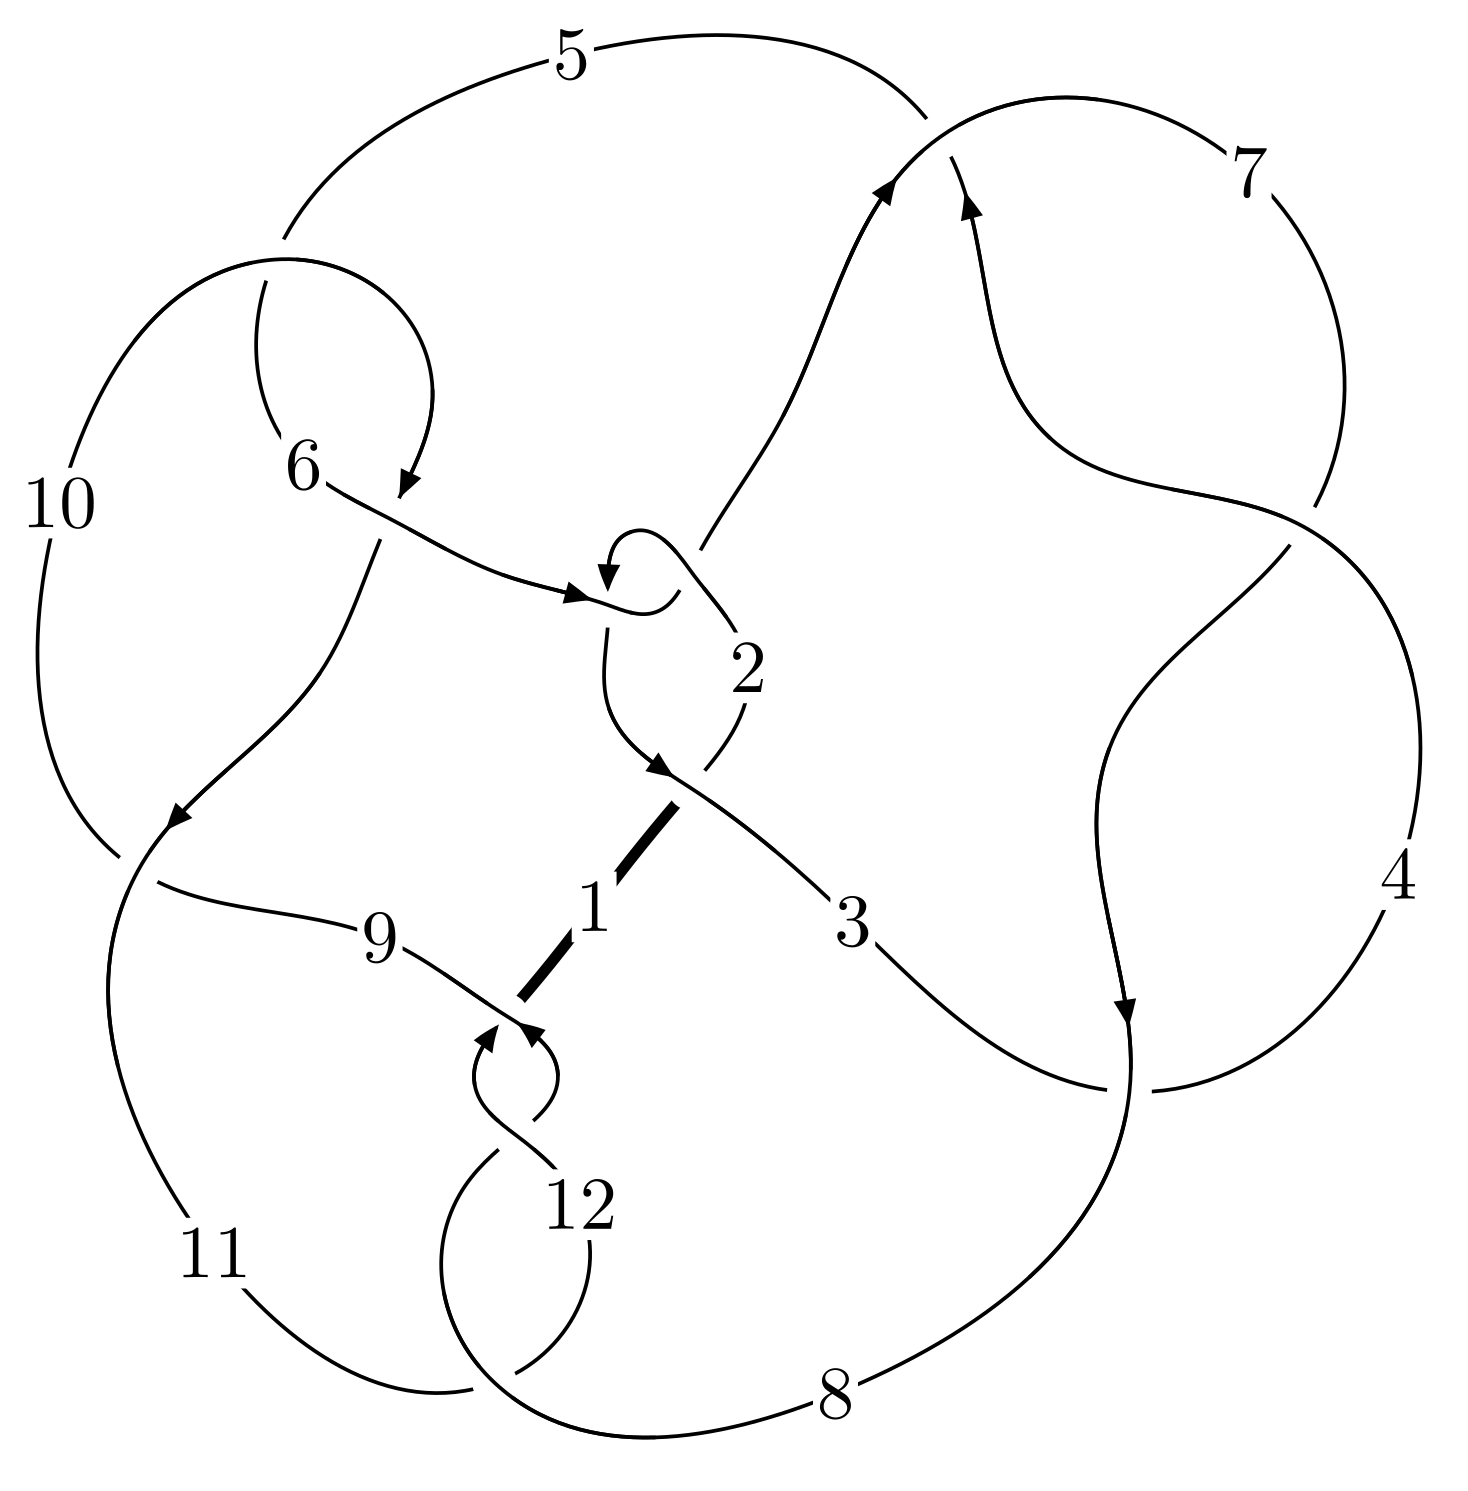
\includegraphics[width=112pt]{../../../GIT/diagram.site/Diagrams/png/2420_12n_0331.png}\\
\ \ \ A knot diagram\footnotemark}&
\allowdisplaybreaks
\textbf{Linearized knot diagam} \\
\cline{2-2}
 &
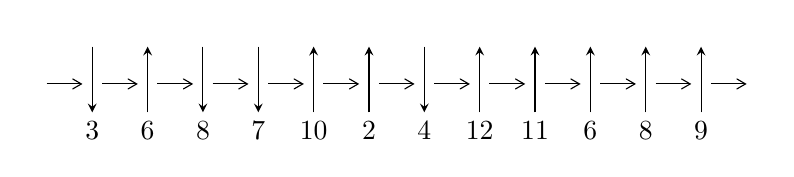
\begin{tikzpicture}[x=20pt, y=17pt]
	% nodes
	\node (C0) at (0, 0) {};
	\node (C1) at (1, 0) {};
	\node (C1U) at (1, +1) {};
	\node (C1D) at (1, -1) {3};

	\node (C2) at (2, 0) {};
	\node (C2U) at (2, +1) {};
	\node (C2D) at (2, -1) {6};

	\node (C3) at (3, 0) {};
	\node (C3U) at (3, +1) {};
	\node (C3D) at (3, -1) {8};

	\node (C4) at (4, 0) {};
	\node (C4U) at (4, +1) {};
	\node (C4D) at (4, -1) {7};

	\node (C5) at (5, 0) {};
	\node (C5U) at (5, +1) {};
	\node (C5D) at (5, -1) {10};

	\node (C6) at (6, 0) {};
	\node (C6U) at (6, +1) {};
	\node (C6D) at (6, -1) {2};

	\node (C7) at (7, 0) {};
	\node (C7U) at (7, +1) {};
	\node (C7D) at (7, -1) {4};

	\node (C8) at (8, 0) {};
	\node (C8U) at (8, +1) {};
	\node (C8D) at (8, -1) {12};

	\node (C9) at (9, 0) {};
	\node (C9U) at (9, +1) {};
	\node (C9D) at (9, -1) {11};

	\node (C10) at (10, 0) {};
	\node (C10U) at (10, +1) {};
	\node (C10D) at (10, -1) {6};

	\node (C11) at (11, 0) {};
	\node (C11U) at (11, +1) {};
	\node (C11D) at (11, -1) {8};

	\node (C12) at (12, 0) {};
	\node (C12U) at (12, +1) {};
	\node (C12D) at (12, -1) {9};
	\node (C13) at (13, 0) {};

	% arrows
	\draw[->,>={angle 60}]
	(C0) edge (C1) (C1) edge (C2) (C2) edge (C3) (C3) edge (C4) (C4) edge (C5) (C5) edge (C6) (C6) edge (C7) (C7) edge (C8) (C8) edge (C9) (C9) edge (C10) (C10) edge (C11) (C11) edge (C12) (C12) edge (C13) ;	\draw[->,>=stealth]
	(C1U) edge (C1D) (C2D) edge (C2U) (C3U) edge (C3D) (C4U) edge (C4D) (C5D) edge (C5U) (C6D) edge (C6U) (C7U) edge (C7D) (C8D) edge (C8U) (C9D) edge (C9U) (C10D) edge (C10U) (C11D) edge (C11U) (C12D) edge (C12U) ;
	\end{tikzpicture} \\
\hhline{~~} \\& 
\textbf{Solving Sequence} \\ \cline{2-2} 
 &
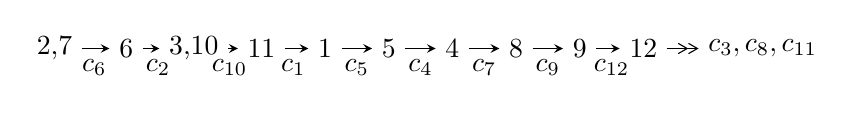
\begin{tikzpicture}[x=23pt, y=7pt]
	% node
	\node (A0) at (-1/8, 0) {2,7};
	\node (A1) at (1, 0) {6};
	\node (A2) at (33/16, 0) {3,10};
	\node (A3) at (25/8, 0) {11};
	\node (A4) at (33/8, 0) {1};
	\node (A5) at (41/8, 0) {5};
	\node (A6) at (49/8, 0) {4};
	\node (A7) at (57/8, 0) {8};
	\node (A8) at (65/8, 0) {9};
	\node (A9) at (73/8, 0) {12};
	\node (C1) at (1/2, -1) {$c_{6}$};
	\node (C2) at (3/2, -1) {$c_{2}$};
	\node (C3) at (21/8, -1) {$c_{10}$};
	\node (C4) at (29/8, -1) {$c_{1}$};
	\node (C5) at (37/8, -1) {$c_{5}$};
	\node (C6) at (45/8, -1) {$c_{4}$};
	\node (C7) at (53/8, -1) {$c_{7}$};
	\node (C8) at (61/8, -1) {$c_{9}$};
	\node (C9) at (69/8, -1) {$c_{12}$};
	\node (A10) at (11, 0) {$c_{3},c_{8},c_{11}$};

	% edge
	\draw[->,>=stealth]	
	(A0) edge (A1) (A1) edge (A2) (A2) edge (A3) (A3) edge (A4) (A4) edge (A5) (A5) edge (A6) (A6) edge (A7) (A7) edge (A8) (A8) edge (A9) ;
	\draw[->>,>={angle 60}]	
	(A9) edge (A10);
\end{tikzpicture} \\ 

\end{tabular} \\

\footnotetext{
The image of knot diagram is generated by the software ``\textbf{Draw programme}" developed by Andrew Bartholomew(\url{http://www.layer8.co.uk/maths/draw/index.htm\#Running-draw}), where we modified some parts for our purpose(\url{https://github.com/CATsTAILs/LinksPainter}).
}\phantom \\ \newline 
\centering \textbf{Ideals for irreducible components\footnotemark of $X_{\text{par}}$} 
 
\begin{align*}
I^u_{1}&=\langle 
-1.19705\times10^{30} u^{29}+3.06307\times10^{30} u^{28}+\cdots+1.34207\times10^{30} b-3.67175\times10^{31},\\
\phantom{I^u_{1}}&\phantom{= \langle  }-3.01996\times10^{31} u^{29}+7.71851\times10^{31} u^{28}+\cdots+2.28151\times10^{31} a-8.92737\times10^{32},\\
\phantom{I^u_{1}}&\phantom{= \langle  }u^{30}-2 u^{29}+\cdots+54 u+17\rangle \\
I^u_{2}&=\langle 
19 a^4 u+83 a^4-123 a^3 u+119 a^3+186 a^2 u+202 a^2-333 a u+145 b+499 a-9 u-253,\\
\phantom{I^u_{2}}&\phantom{= \langle  }a^5-2 a^4 u+a^4+2 a^3 u+2 a^3-5 a^2 u+4 a^2+a u-6 a+1,\;u^2+1\rangle \\
I^u_{3}&=\langle 
- u^3+2 b+u+1,\;- u^3-2 u^2+2 a-3 u-1,\;u^4+u^3+u^2+1\rangle \\
I^u_{4}&=\langle 
- u^5+u^4- u^3+3 u^2+b-2 u,\;- u^4- u^3- u^2+a+u+2,\;u^6+2 u^4-3 u^3+u^2-3 u+1\rangle \\
\\
\end{align*}
\raggedright * 4 irreducible components of $\dim_{\mathbb{C}}=0$, with total 50 representations.\\
\footnotetext{All coefficients of polynomials are rational numbers. But the coefficients are sometimes approximated in decimal forms when there is not enough margin.}
\newpage
\renewcommand{\arraystretch}{1}
\centering \section*{I. $I^u_{1}= \langle -1.20\times10^{30} u^{29}+3.06\times10^{30} u^{28}+\cdots+1.34\times10^{30} b-3.67\times10^{31},\;-3.02\times10^{31} u^{29}+7.72\times10^{31} u^{28}+\cdots+2.28\times10^{31} a-8.93\times10^{32},\;u^{30}-2 u^{29}+\cdots+54 u+17 \rangle$}
\flushleft \textbf{(i) Arc colorings}\\
\begin{tabular}{m{7pt} m{180pt} m{7pt} m{180pt} }
\flushright $a_{2}=$&$\begin{pmatrix}0\\u\end{pmatrix}$ \\
\flushright $a_{7}=$&$\begin{pmatrix}1\\0\end{pmatrix}$ \\
\flushright $a_{6}=$&$\begin{pmatrix}1\\u^2\end{pmatrix}$ \\
\flushright $a_{3}=$&$\begin{pmatrix}u\\u^3+u\end{pmatrix}$ \\
\flushright $a_{10}=$&$\begin{pmatrix}1.32367 u^{29}-3.38307 u^{28}+\cdots+56.8890 u+39.1292\\0.891947 u^{29}-2.28235 u^{28}+\cdots+38.3521 u+27.3589\end{pmatrix}$ \\
\flushright $a_{11}=$&$\begin{pmatrix}1.81045 u^{29}-4.61918 u^{28}+\cdots+78.0139 u+53.9806\\1.03280 u^{29}-2.64107 u^{28}+\cdots+44.2541 u+31.8222\end{pmatrix}$ \\
\flushright $a_{1}=$&$\begin{pmatrix}u^3\\u^5+u^3+u\end{pmatrix}$ \\
\flushright $a_{5}=$&$\begin{pmatrix}0.469748 u^{29}-1.23844 u^{28}+\cdots+19.5553 u+13.1538\\1.06033 u^{29}-2.72603 u^{28}+\cdots+44.9653 u+31.7036\end{pmatrix}$ \\
\flushright $a_{4}=$&$\begin{pmatrix}1.53008 u^{29}-3.96448 u^{28}+\cdots+64.5205 u+44.8574\\1.06033 u^{29}-2.72603 u^{28}+\cdots+44.9653 u+31.7036\end{pmatrix}$ \\
\flushright $a_{8}=$&$\begin{pmatrix}-0.960602 u^{29}+2.44978 u^{28}+\cdots-40.1263 u-29.7290\\0.605372 u^{29}-1.56263 u^{28}+\cdots+25.5542 u+17.0256\end{pmatrix}$ \\
\flushright $a_{9}=$&$\begin{pmatrix}0.804706 u^{29}-2.05555 u^{28}+\cdots+34.2505 u+23.3776\\-0.518550 u^{29}+1.32875 u^{28}+\cdots-22.1403 u-15.5691\end{pmatrix}$ \\
\flushright $a_{12}=$&$\begin{pmatrix}0.580383 u^{29}-1.46053 u^{28}+\cdots+25.3284 u+18.2709\\0.354478 u^{29}-0.902566 u^{28}+\cdots+15.0764 u+11.6477\end{pmatrix}$\\&\end{tabular}
\flushleft \textbf{(ii) Obstruction class $= -1$}\\~\\
\flushleft \textbf{(iii) Cusp Shapes $= -2.31952 u^{29}+6.05662 u^{28}+\cdots-101.386 u-62.1980$}\\~\\
\newpage\renewcommand{\arraystretch}{1}
\flushleft \textbf{(iv) u-Polynomials at the component}\newline \\
\begin{tabular}{m{50pt}|m{274pt}}
Crossings & \hspace{64pt}u-Polynomials at each crossing \\
\hline $$\begin{aligned}c_{1}\end{aligned}$$&$\begin{aligned}
&u^{30}+36 u^{28}+\cdots-842 u+289
\end{aligned}$\\
\hline $$\begin{aligned}c_{2},c_{6}\end{aligned}$$&$\begin{aligned}
&u^{30}-2 u^{29}+\cdots+54 u+17
\end{aligned}$\\
\hline $$\begin{aligned}c_{3},c_{4},c_{7}\end{aligned}$$&$\begin{aligned}
&u^{30}-2 u^{29}+\cdots+134 u+17
\end{aligned}$\\
\hline $$\begin{aligned}c_{5},c_{10}\end{aligned}$$&$\begin{aligned}
&u^{30}-2 u^{29}+\cdots-16 u+64
\end{aligned}$\\
\hline $$\begin{aligned}c_{8},c_{11},c_{12}\end{aligned}$$&$\begin{aligned}
&u^{30}+4 u^{29}+\cdots+35 u+4
\end{aligned}$\\
\hline $$\begin{aligned}c_{9}\end{aligned}$$&$\begin{aligned}
&u^{30}-24 u^{29}+\cdots+37632 u+4096
\end{aligned}$\\
\hline
\end{tabular}\\~\\
\newpage\renewcommand{\arraystretch}{1}
\flushleft \textbf{(v) Riley Polynomials at the component}\newline \\
\begin{tabular}{m{50pt}|m{274pt}}
Crossings & \hspace{64pt}Riley Polynomials at each crossing \\
\hline $$\begin{aligned}c_{1}\end{aligned}$$&$\begin{aligned}
&y^{30}+72 y^{29}+\cdots-1286386 y+83521
\end{aligned}$\\
\hline $$\begin{aligned}c_{2},c_{6}\end{aligned}$$&$\begin{aligned}
&y^{30}+36 y^{28}+\cdots-842 y+289
\end{aligned}$\\
\hline $$\begin{aligned}c_{3},c_{4},c_{7}\end{aligned}$$&$\begin{aligned}
&y^{30}+48 y^{29}+\cdots+1526 y+289
\end{aligned}$\\
\hline $$\begin{aligned}c_{5},c_{10}\end{aligned}$$&$\begin{aligned}
&y^{30}-24 y^{29}+\cdots+37632 y+4096
\end{aligned}$\\
\hline $$\begin{aligned}c_{8},c_{11},c_{12}\end{aligned}$$&$\begin{aligned}
&y^{30}-32 y^{29}+\cdots-785 y+16
\end{aligned}$\\
\hline $$\begin{aligned}c_{9}\end{aligned}$$&$\begin{aligned}
&y^{30}-44 y^{29}+\cdots-830537728 y+16777216
\end{aligned}$\\
\hline
\end{tabular}\\~\\
\newpage\flushleft \textbf{(vi) Complex Volumes and Cusp Shapes}
$$\begin{array}{c|c|c}  
\text{Solutions to }I^u_{1}& \I (\text{vol} + \sqrt{-1}CS) & \text{Cusp shape}\\
 \hline 
\begin{aligned}
u &= -0.829037 + 0.437570 I \\
a &= \phantom{-}2.03295 + 0.07010 I \\
b &= -0.12264 - 1.43896 I\end{aligned}
 & \phantom{-}3.48161 - 3.37472 I & \phantom{-}9.82032 + 5.06127 I \\ \hline\begin{aligned}
u &= -0.829037 - 0.437570 I \\
a &= \phantom{-}2.03295 - 0.07010 I \\
b &= -0.12264 + 1.43896 I\end{aligned}
 & \phantom{-}3.48161 + 3.37472 I & \phantom{-}9.82032 - 5.06127 I \\ \hline\begin{aligned}
u &= \phantom{-}0.126583 + 0.923400 I \\
a &= \phantom{-}0.197805 - 0.967738 I \\
b &= -0.642069 + 0.460134 I\end{aligned}
 & -1.43679 + 1.72806 I & -2.66066 - 5.45071 I \\ \hline\begin{aligned}
u &= \phantom{-}0.126583 - 0.923400 I \\
a &= \phantom{-}0.197805 + 0.967738 I \\
b &= -0.642069 - 0.460134 I\end{aligned}
 & -1.43679 - 1.72806 I & -2.66066 + 5.45071 I \\ \hline\begin{aligned}
u &= \phantom{-}0.186023 + 1.138800 I \\
a &= \phantom{-}0.312069 + 0.834385 I \\
b &= \phantom{-}0.489861 - 0.585323 I\end{aligned}
 & \phantom{-}3.94202 + 3.99509 I & \phantom{-}4.27681 - 3.33940 I \\ \hline\begin{aligned}
u &= \phantom{-}0.186023 - 1.138800 I \\
a &= \phantom{-}0.312069 - 0.834385 I \\
b &= \phantom{-}0.489861 + 0.585323 I\end{aligned}
 & \phantom{-}3.94202 - 3.99509 I & \phantom{-}4.27681 + 3.33940 I \\ \hline\begin{aligned}
u &= \phantom{-}0.776216 + 0.200551 I \\
a &= -0.122985 + 0.288246 I \\
b &= -0.437118 - 1.021360 I\end{aligned}
 & \phantom{-}5.08101 + 0.72288 I & \phantom{-}10.46952 - 1.61581 I \\ \hline\begin{aligned}
u &= \phantom{-}0.776216 - 0.200551 I \\
a &= -0.122985 - 0.288246 I \\
b &= -0.437118 + 1.021360 I\end{aligned}
 & \phantom{-}5.08101 - 0.72288 I & \phantom{-}10.46952 + 1.61581 I \\ \hline\begin{aligned}
u &= -0.100734 + 0.756568 I \\
a &= -1.29597 + 1.74435 I \\
b &= \phantom{-}1.38516 - 0.30781 I\end{aligned}
 & \phantom{-}1.052880 - 0.788287 I & \phantom{-}1.82250 - 2.44795 I \\ \hline\begin{aligned}
u &= -0.100734 - 0.756568 I \\
a &= -1.29597 - 1.74435 I \\
b &= \phantom{-}1.38516 + 0.30781 I\end{aligned}
 & \phantom{-}1.052880 + 0.788287 I & \phantom{-}1.82250 + 2.44795 I\\
 \hline 
 \end{array}$$\newpage$$\begin{array}{c|c|c}  
\text{Solutions to }I^u_{1}& \I (\text{vol} + \sqrt{-1}CS) & \text{Cusp shape}\\
 \hline 
\begin{aligned}
u &= \phantom{-}0.405861 + 0.639492 I \\
a &= -0.273422 - 0.284148 I \\
b &= \phantom{-}0.206163 + 0.373793 I\end{aligned}
 & \phantom{-}0.05508 + 1.46864 I & \phantom{-}0.73396 - 4.75961 I \\ \hline\begin{aligned}
u &= \phantom{-}0.405861 - 0.639492 I \\
a &= -0.273422 + 0.284148 I \\
b &= \phantom{-}0.206163 - 0.373793 I\end{aligned}
 & \phantom{-}0.05508 - 1.46864 I & \phantom{-}0.73396 + 4.75961 I \\ \hline\begin{aligned}
u &= -0.531183 + 0.468483 I \\
a &= \phantom{-}0.20768 + 1.54378 I \\
b &= -0.307002 + 0.554265 I\end{aligned}
 & \phantom{-}7.65219 - 5.07226 I & \phantom{-}12.77738 + 5.27340 I \\ \hline\begin{aligned}
u &= -0.531183 - 0.468483 I \\
a &= \phantom{-}0.20768 - 1.54378 I \\
b &= -0.307002 - 0.554265 I\end{aligned}
 & \phantom{-}7.65219 + 5.07226 I & \phantom{-}12.77738 - 5.27340 I \\ \hline\begin{aligned}
u &= -0.928021 + 0.930066 I \\
a &= \phantom{-}0.284525 + 0.123937 I \\
b &= \phantom{-}0.185780 + 0.143992 I\end{aligned}
 & \phantom{-}7.86055 - 3.38055 I & \phantom{-}1.34955 + 4.07729 I \\ \hline\begin{aligned}
u &= -0.928021 - 0.930066 I \\
a &= \phantom{-}0.284525 - 0.123937 I \\
b &= \phantom{-}0.185780 - 0.143992 I\end{aligned}
 & \phantom{-}7.86055 + 3.38055 I & \phantom{-}1.34955 - 4.07729 I \\ \hline\begin{aligned}
u &= -1.128230 + 0.737366 I \\
a &= -1.42056 - 0.51782 I \\
b &= -0.24507 + 1.51911 I\end{aligned}
 & \phantom{-}11.39290 - 6.89335 I & \phantom{-}10.03435 + 4.47976 I \\ \hline\begin{aligned}
u &= -1.128230 - 0.737366 I \\
a &= -1.42056 + 0.51782 I \\
b &= -0.24507 - 1.51911 I\end{aligned}
 & \phantom{-}11.39290 + 6.89335 I & \phantom{-}10.03435 - 4.47976 I \\ \hline\begin{aligned}
u &= -0.566721 + 0.006749 I \\
a &= -1.95664 + 1.43740 I \\
b &= \phantom{-}0.389339 + 0.933911 I\end{aligned}
 & \phantom{-}2.43486 + 1.42637 I & \phantom{-}9.21244 - 2.51396 I \\ \hline\begin{aligned}
u &= -0.566721 - 0.006749 I \\
a &= -1.95664 - 1.43740 I \\
b &= \phantom{-}0.389339 - 0.933911 I\end{aligned}
 & \phantom{-}2.43486 - 1.42637 I & \phantom{-}9.21244 + 2.51396 I\\
 \hline 
 \end{array}$$\newpage$$\begin{array}{c|c|c}  
\text{Solutions to }I^u_{1}& \I (\text{vol} + \sqrt{-1}CS) & \text{Cusp shape}\\
 \hline 
\begin{aligned}
u &= \phantom{-}1.22801 + 1.05643 I \\
a &= \phantom{-}1.121090 - 0.442399 I \\
b &= \phantom{-}0.00806 + 2.83114 I\end{aligned}
 & \phantom{-}13.79620 + 0.94673 I & \phantom{-}9.08350 + 0. I\phantom{ +0.000000I} \\ \hline\begin{aligned}
u &= \phantom{-}1.22801 - 1.05643 I \\
a &= \phantom{-}1.121090 + 0.442399 I \\
b &= \phantom{-}0.00806 - 2.83114 I\end{aligned}
 & \phantom{-}13.79620 - 0.94673 I & \phantom{-}9.08350 + 0. I\phantom{ +0.000000I} \\ \hline\begin{aligned}
u &= \phantom{-}1.10289 + 1.19850 I \\
a &= -1.146390 + 0.819322 I \\
b &= -0.38922 - 2.83191 I\end{aligned}
 & \phantom{-}13.2760 + 7.5606 I & \phantom{-}8.25231 - 4.41681 I \\ \hline\begin{aligned}
u &= \phantom{-}1.10289 - 1.19850 I \\
a &= -1.146390 - 0.819322 I \\
b &= -0.38922 + 2.83191 I\end{aligned}
 & \phantom{-}13.2760 - 7.5606 I & \phantom{-}8.25231 + 4.41681 I \\ \hline\begin{aligned}
u &= -1.18793 + 1.15252 I \\
a &= -0.518013 - 0.112474 I \\
b &= -0.508297 - 0.220564 I\end{aligned}
 & \phantom{-}15.8822 - 4.3416 I & \phantom{-}9.48749 + 2.02953 I \\ \hline\begin{aligned}
u &= -1.18793 - 1.15252 I \\
a &= -0.518013 + 0.112474 I \\
b &= -0.508297 + 0.220564 I\end{aligned}
 & \phantom{-}15.8822 + 4.3416 I & \phantom{-}9.48749 - 2.02953 I \\ \hline\begin{aligned}
u &= \phantom{-}1.00823 + 1.34227 I \\
a &= \phantom{-}0.94025 - 1.06187 I \\
b &= \phantom{-}0.56557 + 2.56886 I\end{aligned}
 & -19.2136 + 12.8082 I & \phantom{-}9.69103 - 5.43858 I \\ \hline\begin{aligned}
u &= \phantom{-}1.00823 - 1.34227 I \\
a &= \phantom{-}0.94025 + 1.06187 I \\
b &= \phantom{-}0.56557 - 2.56886 I\end{aligned}
 & -19.2136 - 12.8082 I & \phantom{-}9.69103 + 5.43858 I \\ \hline\begin{aligned}
u &= \phantom{-}1.43803 + 0.89416 I \\
a &= -0.818277 + 0.222471 I \\
b &= \phantom{-}0.17149 - 2.49018 I\end{aligned}
 & -17.5541 - 4.0475 I & \phantom{-}10.77450 + 0. I\phantom{ +0.000000I} \\ \hline\begin{aligned}
u &= \phantom{-}1.43803 - 0.89416 I \\
a &= -0.818277 - 0.222471 I \\
b &= \phantom{-}0.17149 + 2.49018 I\end{aligned}
 & -17.5541 + 4.0475 I & \phantom{-}10.77450 + 0. I\phantom{ +0.000000I}\\
 \hline 
 \end{array}$$\newpage\newpage\renewcommand{\arraystretch}{1}
\centering \section*{II. $I^u_{2}= \langle 19 a^4 u-123 a^3 u+\cdots+499 a-253,\;-2 a^4 u+2 a^3 u+\cdots-6 a+1,\;u^2+1 \rangle$}
\flushleft \textbf{(i) Arc colorings}\\
\begin{tabular}{m{7pt} m{180pt} m{7pt} m{180pt} }
\flushright $a_{2}=$&$\begin{pmatrix}0\\u\end{pmatrix}$ \\
\flushright $a_{7}=$&$\begin{pmatrix}1\\0\end{pmatrix}$ \\
\flushright $a_{6}=$&$\begin{pmatrix}1\\-1\end{pmatrix}$ \\
\flushright $a_{3}=$&$\begin{pmatrix}u\\0\end{pmatrix}$ \\
\flushright $a_{10}=$&$\begin{pmatrix}a\\-0.131034 a^{4} u+0.848276 a^{3} u+\cdots-3.44138 a+1.74483\end{pmatrix}$ \\
\flushright $a_{11}=$&$\begin{pmatrix}-0.131034 a^{4} u+0.848276 a^{3} u+\cdots-1.44138 a+1.74483\\- a\end{pmatrix}$ \\
\flushright $a_{1}=$&$\begin{pmatrix}- u\\u\end{pmatrix}$ \\
\flushright $a_{5}=$&$\begin{pmatrix}-0.165517 a^{4} u+0.124138 a^{3} u+\cdots-1.82069 a+1.57241\\u\end{pmatrix}$ \\
\flushright $a_{4}=$&$\begin{pmatrix}-0.165517 a^{4} u+0.124138 a^{3} u+\cdots-1.82069 a+1.57241\\u\end{pmatrix}$ \\
\flushright $a_{8}=$&$\begin{pmatrix}0.0137931 a^{4} u-0.510345 a^{3} u+\cdots+0.151724 a-0.131034\\-1\end{pmatrix}$ \\
\flushright $a_{9}=$&$\begin{pmatrix}0.0689655 a^{4} u-0.551724 a^{3} u+\cdots+2.75862 a-1.65517\\0.186207 a^{4} u+1.11034 a^{3} u+\cdots-1.95172 a+1.73103\end{pmatrix}$ \\
\flushright $a_{12}=$&$\begin{pmatrix}-0.275862 a^{4} u+0.206897 a^{3} u+\cdots-3.03448 a+1.62069\\-0.0620690 a^{4} u-0.703448 a^{3} u+\cdots+1.31724 a-1.91034\end{pmatrix}$\\&\end{tabular}
\flushleft \textbf{(ii) Obstruction class $= 1$}\\~\\
\flushleft \textbf{(iii) Cusp Shapes $= \frac{132}{145} a^4 u-\frac{156}{145} a^4+\frac{336}{145} a^3 u-\frac{28}{145} a^3-\frac{112}{145} a^2 u-\frac{764}{145} a^2+\frac{556}{145} a u-\frac{288}{145} a-\frac{612}{145} u+\frac{1356}{145}$}\\~\\
\newpage\renewcommand{\arraystretch}{1}
\flushleft \textbf{(iv) u-Polynomials at the component}\newline \\
\begin{tabular}{m{50pt}|m{274pt}}
Crossings & \hspace{64pt}u-Polynomials at each crossing \\
\hline $$\begin{aligned}c_{1}\end{aligned}$$&$\begin{aligned}
&(u-1)^{10}
\end{aligned}$\\
\hline $$\begin{aligned}c_{2},c_{3},c_{4}\\c_{6},c_{7}\end{aligned}$$&$\begin{aligned}
&(u^2+1)^5
\end{aligned}$\\
\hline $$\begin{aligned}c_{5},c_{10}\end{aligned}$$&$\begin{aligned}
&u^{10}-3 u^8+4 u^6- u^4- u^2+1
\end{aligned}$\\
\hline $$\begin{aligned}c_{8}\end{aligned}$$&$\begin{aligned}
&(u^5- u^4-2 u^3+u^2+u+1)^2
\end{aligned}$\\
\hline $$\begin{aligned}c_{9}\end{aligned}$$&$\begin{aligned}
&(u^5+3 u^4+4 u^3+u^2- u-1)^2
\end{aligned}$\\
\hline $$\begin{aligned}c_{11},c_{12}\end{aligned}$$&$\begin{aligned}
&(u^5+u^4-2 u^3- u^2+u-1)^2
\end{aligned}$\\
\hline
\end{tabular}\\~\\
\newpage\renewcommand{\arraystretch}{1}
\flushleft \textbf{(v) Riley Polynomials at the component}\newline \\
\begin{tabular}{m{50pt}|m{274pt}}
Crossings & \hspace{64pt}Riley Polynomials at each crossing \\
\hline $$\begin{aligned}c_{1}\end{aligned}$$&$\begin{aligned}
&(y-1)^{10}
\end{aligned}$\\
\hline $$\begin{aligned}c_{2},c_{3},c_{4}\\c_{6},c_{7}\end{aligned}$$&$\begin{aligned}
&(y+1)^{10}
\end{aligned}$\\
\hline $$\begin{aligned}c_{5},c_{10}\end{aligned}$$&$\begin{aligned}
&(y^5-3 y^4+4 y^3- y^2- y+1)^2
\end{aligned}$\\
\hline $$\begin{aligned}c_{8},c_{11},c_{12}\end{aligned}$$&$\begin{aligned}
&(y^5-5 y^4+8 y^3-3 y^2- y-1)^2
\end{aligned}$\\
\hline $$\begin{aligned}c_{9}\end{aligned}$$&$\begin{aligned}
&(y^5- y^4+8 y^3-3 y^2+3 y-1)^2
\end{aligned}$\\
\hline
\end{tabular}\\~\\
\newpage\flushleft \textbf{(vi) Complex Volumes and Cusp Shapes}
$$\begin{array}{c|c|c}  
\text{Solutions to }I^u_{2}& \I (\text{vol} + \sqrt{-1}CS) & \text{Cusp shape}\\
 \hline 
\begin{aligned}
u &= \phantom{-0.000000 -}1.000000 I \\
a &= \phantom{-}0.645450 + 0.271616 I \\
b &= -1.46782 - 0.61073 I\end{aligned}
 & \phantom{-}0.32910 + 1.53058 I & \phantom{-}4.51511 - 4.43065 I \\ \hline\begin{aligned}
u &= \phantom{-0.000000 -}1.000000 I \\
a &= -0.74843 + 1.46044 I \\
b &= -0.451726 - 1.004750 I\end{aligned}
 & \phantom{-}5.87256 - 4.40083 I & \phantom{-}8.74431 + 3.49859 I \\ \hline\begin{aligned}
u &= \phantom{-0.000000 -}1.000000 I \\
a &= \phantom{-}0.195404 + 0.003972 I \\
b &= \phantom{-}1.004750 + 0.451726 I\end{aligned}
 & \phantom{-}5.87256 + 4.40083 I & \phantom{-}8.74431 - 3.49859 I \\ \hline\begin{aligned}
u &= \phantom{-0.000000 -}1.000000 I \\
a &= \phantom{-}0.21165 - 1.80694 I \\
b &= \phantom{-}0.61073 + 1.46782 I\end{aligned}
 & \phantom{-}0.32910 - 1.53058 I & \phantom{-}4.51511 + 4.43065 I \\ \hline\begin{aligned}
u &= \phantom{-0.000000 -}1.000000 I \\
a &= -1.30408 + 2.07090 I \\
b &= \phantom{-}1.30408 - 1.30408 I\end{aligned}
 & \phantom{-}2.40108\phantom{ +0.000000I} & \phantom{-}5.48114 + 0. I\phantom{ +0.000000I} \\ \hline\begin{aligned}
u &= \phantom{-0.000000 } -1.000000 I \\
a &= \phantom{-}0.645450 - 0.271616 I \\
b &= -1.46782 + 0.61073 I\end{aligned}
 & \phantom{-}0.32910 - 1.53058 I & \phantom{-}4.51511 + 4.43065 I \\ \hline\begin{aligned}
u &= \phantom{-0.000000 } -1.000000 I \\
a &= -0.74843 - 1.46044 I \\
b &= -0.451726 + 1.004750 I\end{aligned}
 & \phantom{-}5.87256 + 4.40083 I & \phantom{-}8.74431 - 3.49859 I \\ \hline\begin{aligned}
u &= \phantom{-0.000000 } -1.000000 I \\
a &= \phantom{-}0.195404 - 0.003972 I \\
b &= \phantom{-}1.004750 - 0.451726 I\end{aligned}
 & \phantom{-}5.87256 - 4.40083 I & \phantom{-}8.74431 + 3.49859 I \\ \hline\begin{aligned}
u &= \phantom{-0.000000 } -1.000000 I \\
a &= \phantom{-}0.21165 + 1.80694 I \\
b &= \phantom{-}0.61073 - 1.46782 I\end{aligned}
 & \phantom{-}0.32910 + 1.53058 I & \phantom{-}4.51511 - 4.43065 I \\ \hline\begin{aligned}
u &= \phantom{-0.000000 } -1.000000 I \\
a &= -1.30408 - 2.07090 I \\
b &= \phantom{-}1.30408 + 1.30408 I\end{aligned}
 & \phantom{-}2.40108\phantom{ +0.000000I} & \phantom{-}5.48114 + 0. I\phantom{ +0.000000I}\\
 \hline 
 \end{array}$$\newpage\newpage\renewcommand{\arraystretch}{1}
\centering \section*{III. $I^u_{3}= \langle - u^3+2 b+u+1,\;- u^3-2 u^2+2 a-3 u-1,\;u^4+u^3+u^2+1 \rangle$}
\flushleft \textbf{(i) Arc colorings}\\
\begin{tabular}{m{7pt} m{180pt} m{7pt} m{180pt} }
\flushright $a_{2}=$&$\begin{pmatrix}0\\u\end{pmatrix}$ \\
\flushright $a_{7}=$&$\begin{pmatrix}1\\0\end{pmatrix}$ \\
\flushright $a_{6}=$&$\begin{pmatrix}1\\u^2\end{pmatrix}$ \\
\flushright $a_{3}=$&$\begin{pmatrix}u\\u^3+u\end{pmatrix}$ \\
\flushright $a_{10}=$&$\begin{pmatrix}\frac{1}{2} u^3+u^2+\frac{3}{2} u+\frac{1}{2}\\\frac{1}{2} u^3-\frac{1}{2} u-\frac{1}{2}\end{pmatrix}$ \\
\flushright $a_{11}=$&$\begin{pmatrix}\frac{1}{2} u^3+u^2+\frac{3}{2} u+\frac{1}{2}\\\frac{1}{2} u^3-\frac{1}{2} u-\frac{1}{2}\end{pmatrix}$ \\
\flushright $a_{1}=$&$\begin{pmatrix}u^3\\u^3+u^2+1\end{pmatrix}$ \\
\flushright $a_{5}=$&$\begin{pmatrix}1\\u^2\end{pmatrix}$ \\
\flushright $a_{4}=$&$\begin{pmatrix}u^2+1\\u^2\end{pmatrix}$ \\
\flushright $a_{8}=$&$\begin{pmatrix}- u^3\\- u^3- u^2-1\end{pmatrix}$ \\
\flushright $a_{9}=$&$\begin{pmatrix}\frac{1}{2} u^3+u^2+\frac{3}{2} u+\frac{1}{2}\\\frac{1}{2} u^3-\frac{1}{2} u-\frac{1}{2}\end{pmatrix}$ \\
\flushright $a_{12}=$&$\begin{pmatrix}\frac{3}{2} u^3+u^2+\frac{3}{2} u+\frac{1}{2}\\\frac{3}{2} u^3+u^2-\frac{1}{2} u+\frac{1}{2}\end{pmatrix}$\\&\end{tabular}
\flushleft \textbf{(ii) Obstruction class $= 1$}\\~\\
\flushleft \textbf{(iii) Cusp Shapes $= -\frac{1}{4} u^3-\frac{7}{2} u^2-\frac{23}{4} u+\frac{37}{4}$}\\~\\
\newpage\renewcommand{\arraystretch}{1}
\flushleft \textbf{(iv) u-Polynomials at the component}\newline \\
\begin{tabular}{m{50pt}|m{274pt}}
Crossings & \hspace{64pt}u-Polynomials at each crossing \\
\hline $$\begin{aligned}c_{1},c_{3},c_{4}\end{aligned}$$&$\begin{aligned}
&u^4- u^3+3 u^2-2 u+1
\end{aligned}$\\
\hline $$\begin{aligned}c_{2}\end{aligned}$$&$\begin{aligned}
&u^4- u^3+u^2+1
\end{aligned}$\\
\hline $$\begin{aligned}c_{5},c_{9},c_{10}\end{aligned}$$&$\begin{aligned}
&u^4
\end{aligned}$\\
\hline $$\begin{aligned}c_{6}\end{aligned}$$&$\begin{aligned}
&u^4+u^3+u^2+1
\end{aligned}$\\
\hline $$\begin{aligned}c_{7}\end{aligned}$$&$\begin{aligned}
&u^4+u^3+3 u^2+2 u+1
\end{aligned}$\\
\hline $$\begin{aligned}c_{8}\end{aligned}$$&$\begin{aligned}
&(u+1)^4
\end{aligned}$\\
\hline $$\begin{aligned}c_{11},c_{12}\end{aligned}$$&$\begin{aligned}
&(u-1)^4
\end{aligned}$\\
\hline
\end{tabular}\\~\\
\newpage\renewcommand{\arraystretch}{1}
\flushleft \textbf{(v) Riley Polynomials at the component}\newline \\
\begin{tabular}{m{50pt}|m{274pt}}
Crossings & \hspace{64pt}Riley Polynomials at each crossing \\
\hline $$\begin{aligned}c_{1},c_{3},c_{4}\\c_{7}\end{aligned}$$&$\begin{aligned}
&y^4+5 y^3+7 y^2+2 y+1
\end{aligned}$\\
\hline $$\begin{aligned}c_{2},c_{6}\end{aligned}$$&$\begin{aligned}
&y^4+y^3+3 y^2+2 y+1
\end{aligned}$\\
\hline $$\begin{aligned}c_{5},c_{9},c_{10}\end{aligned}$$&$\begin{aligned}
&y^4
\end{aligned}$\\
\hline $$\begin{aligned}c_{8},c_{11},c_{12}\end{aligned}$$&$\begin{aligned}
&(y-1)^4
\end{aligned}$\\
\hline
\end{tabular}\\~\\
\newpage\flushleft \textbf{(vi) Complex Volumes and Cusp Shapes}
$$\begin{array}{c|c|c}  
\text{Solutions to }I^u_{3}& \I (\text{vol} + \sqrt{-1}CS) & \text{Cusp shape}\\
 \hline 
\begin{aligned}
u &= \phantom{-}0.351808 + 0.720342 I \\
a &= \phantom{-}0.38053 + 1.53420 I \\
b &= -0.927958 - 0.413327 I\end{aligned}
 & \phantom{-}1.43393 + 1.41510 I & \phantom{-}8.73606 - 5.88934 I \\ \hline\begin{aligned}
u &= \phantom{-}0.351808 - 0.720342 I \\
a &= \phantom{-}0.38053 - 1.53420 I \\
b &= -0.927958 + 0.413327 I\end{aligned}
 & \phantom{-}1.43393 - 1.41510 I & \phantom{-}8.73606 + 5.88934 I \\ \hline\begin{aligned}
u &= -0.851808 + 0.911292 I \\
a &= -0.130534 + 0.427872 I \\
b &= \phantom{-}0.677958 + 0.157780 I\end{aligned}
 & \phantom{-}8.43568 - 3.16396 I & \phantom{-}14.13894 - 0.11292 I \\ \hline\begin{aligned}
u &= -0.851808 - 0.911292 I \\
a &= -0.130534 - 0.427872 I \\
b &= \phantom{-}0.677958 - 0.157780 I\end{aligned}
 & \phantom{-}8.43568 + 3.16396 I & \phantom{-}14.13894 + 0.11292 I\\
 \hline 
 \end{array}$$\newpage\newpage\renewcommand{\arraystretch}{1}
\centering \section*{IV. $I^u_{4}= \langle - u^5+u^4- u^3+3 u^2+b-2 u,\;- u^4- u^3- u^2+a+u+2,\;u^6+2 u^4-3 u^3+u^2-3 u+1 \rangle$}
\flushleft \textbf{(i) Arc colorings}\\
\begin{tabular}{m{7pt} m{180pt} m{7pt} m{180pt} }
\flushright $a_{2}=$&$\begin{pmatrix}0\\u\end{pmatrix}$ \\
\flushright $a_{7}=$&$\begin{pmatrix}1\\0\end{pmatrix}$ \\
\flushright $a_{6}=$&$\begin{pmatrix}1\\u^2\end{pmatrix}$ \\
\flushright $a_{3}=$&$\begin{pmatrix}u\\u^3+u\end{pmatrix}$ \\
\flushright $a_{10}=$&$\begin{pmatrix}u^4+u^3+u^2- u-2\\u^5- u^4+u^3-3 u^2+2 u\end{pmatrix}$ \\
\flushright $a_{11}=$&$\begin{pmatrix}u^4+u^2-2 u-1\\- u^4-2 u^2+2 u\end{pmatrix}$ \\
\flushright $a_{1}=$&$\begin{pmatrix}u^3\\u^5+u^3+u\end{pmatrix}$ \\
\flushright $a_{5}=$&$\begin{pmatrix}- u\\u\end{pmatrix}$ \\
\flushright $a_{4}=$&$\begin{pmatrix}0\\u\end{pmatrix}$ \\
\flushright $a_{8}=$&$\begin{pmatrix}1\\u^2\end{pmatrix}$ \\
\flushright $a_{9}=$&$\begin{pmatrix}2 u^3+u-2\\2 u^5+2 u^3-2 u^2+u\end{pmatrix}$ \\
\flushright $a_{12}=$&$\begin{pmatrix}u^4- u^3+u^2-3 u\\- u^5- u^4- u^3- u^2+2 u\end{pmatrix}$\\&\end{tabular}
\flushleft \textbf{(ii) Obstruction class $= -1$}\\~\\
\flushleft \textbf{(iii) Cusp Shapes $= 10$}\\~\\
\newpage\renewcommand{\arraystretch}{1}
\flushleft \textbf{(iv) u-Polynomials at the component}\newline \\
\begin{tabular}{m{50pt}|m{274pt}}
Crossings & \hspace{64pt}u-Polynomials at each crossing \\
\hline $$\begin{aligned}c_{1}\end{aligned}$$&$\begin{aligned}
&u^6+4 u^5+6 u^4-3 u^3-13 u^2-7 u+1
\end{aligned}$\\
\hline $$\begin{aligned}c_{2},c_{3},c_{4}\\c_{6},c_{7}\end{aligned}$$&$\begin{aligned}
&u^6+2 u^4-3 u^3+u^2-3 u+1
\end{aligned}$\\
\hline $$\begin{aligned}c_{5},c_{8},c_{10}\\c_{11},c_{12}\end{aligned}$$&$\begin{aligned}
&(u^2+u-1)^3
\end{aligned}$\\
\hline $$\begin{aligned}c_{9}\end{aligned}$$&$\begin{aligned}
&(u^2-3 u+1)^3
\end{aligned}$\\
\hline
\end{tabular}\\~\\
\newpage\renewcommand{\arraystretch}{1}
\flushleft \textbf{(v) Riley Polynomials at the component}\newline \\
\begin{tabular}{m{50pt}|m{274pt}}
Crossings & \hspace{64pt}Riley Polynomials at each crossing \\
\hline $$\begin{aligned}c_{1}\end{aligned}$$&$\begin{aligned}
&y^6-4 y^5+34 y^4-107 y^3+139 y^2-75 y+1
\end{aligned}$\\
\hline $$\begin{aligned}c_{2},c_{3},c_{4}\\c_{6},c_{7}\end{aligned}$$&$\begin{aligned}
&y^6+4 y^5+6 y^4-3 y^3-13 y^2-7 y+1
\end{aligned}$\\
\hline $$\begin{aligned}c_{5},c_{8},c_{10}\\c_{11},c_{12}\end{aligned}$$&$\begin{aligned}
&(y^2-3 y+1)^3
\end{aligned}$\\
\hline $$\begin{aligned}c_{9}\end{aligned}$$&$\begin{aligned}
&(y^2-7 y+1)^3
\end{aligned}$\\
\hline
\end{tabular}\\~\\
\newpage\flushleft \textbf{(vi) Complex Volumes and Cusp Shapes}
$$\begin{array}{c|c|c}  
\text{Solutions to }I^u_{4}& \I (\text{vol} + \sqrt{-1}CS) & \text{Cusp shape}\\
 \hline 
\begin{aligned}
u &= -0.170987 + 1.042930 I \\
a &= -1.34137 - 1.68750 I \\
b &= \phantom{-}1.43598 + 2.26458 I\end{aligned}
 & \phantom{-}0.986960\phantom{ +0.000000I} & \phantom{-}10.0000\phantom{ +0.000000I} \\ \hline\begin{aligned}
u &= -0.170987 - 1.042930 I \\
a &= -1.34137 + 1.68750 I \\
b &= \phantom{-}1.43598 - 2.26458 I\end{aligned}
 & \phantom{-}0.986960\phantom{ +0.000000I} & \phantom{-}10.0000\phantom{ +0.000000I} \\ \hline\begin{aligned}
u &= \phantom{-}1.13928\phantom{ +0.000000I} \\
a &= \phantom{-}1.32215\phantom{ +0.000000I} \\
b &= \phantom{-}0.0980714\phantom{ +0.000000I}\end{aligned}
 & \phantom{-}8.88264\phantom{ +0.000000I} & \phantom{-}10.0000\phantom{ +0.000000I} \\ \hline\begin{aligned}
u &= -0.56964 + 1.40480 I \\
a &= \phantom{-}0.265976 + 0.868217 I \\
b &= -0.66707 - 1.85736 I\end{aligned}
 & \phantom{-}8.88264\phantom{ +0.000000I} & \phantom{-}10.0000\phantom{ +0.000000I} \\ \hline\begin{aligned}
u &= -0.56964 - 1.40480 I \\
a &= \phantom{-}0.265976 - 0.868217 I \\
b &= -0.66707 + 1.85736 I\end{aligned}
 & \phantom{-}8.88264\phantom{ +0.000000I} & \phantom{-}10.0000\phantom{ +0.000000I} \\ \hline\begin{aligned}
u &= \phantom{-}0.341974\phantom{ +0.000000I} \\
a &= -2.17136\phantom{ +0.000000I} \\
b &= \phantom{-}0.364102\phantom{ +0.000000I}\end{aligned}
 & \phantom{-}0.986960\phantom{ +0.000000I} & \phantom{-}10.0000\phantom{ +0.000000I}\\
 \hline 
 \end{array}$$\newpage
\newpage\renewcommand{\arraystretch}{1}
\centering \section*{ V. u-Polynomials}
\begin{tabular}{m{50pt}|m{274pt}}
Crossings & \hspace{64pt}u-Polynomials at each crossing \\
\hline $$\begin{aligned}c_{1}\end{aligned}$$&$\begin{aligned}
&((u-1)^{10})(u^4- u^3+3 u^2-2 u+1)(u^6+4 u^5+\cdots-7 u+1)\\
&\cdot(u^{30}+36 u^{28}+\cdots-842 u+289)
\end{aligned}$\\
\hline $$\begin{aligned}c_{2}\end{aligned}$$&$\begin{aligned}
&(u^2+1)^5(u^4- u^3+u^2+1)(u^6+2 u^4-3 u^3+u^2-3 u+1)\\
&\cdot(u^{30}-2 u^{29}+\cdots+54 u+17)
\end{aligned}$\\
\hline $$\begin{aligned}c_{3},c_{4}\end{aligned}$$&$\begin{aligned}
&(u^2+1)^5(u^4- u^3+3 u^2-2 u+1)(u^6+2 u^4-3 u^3+u^2-3 u+1)\\
&\cdot(u^{30}-2 u^{29}+\cdots+134 u+17)
\end{aligned}$\\
\hline $$\begin{aligned}c_{5},c_{10}\end{aligned}$$&$\begin{aligned}
&u^4(u^2+u-1)^3(u^{10}-3 u^8+4 u^6- u^4- u^2+1)\\
&\cdot(u^{30}-2 u^{29}+\cdots-16 u+64)
\end{aligned}$\\
\hline $$\begin{aligned}c_{6}\end{aligned}$$&$\begin{aligned}
&(u^2+1)^5(u^4+u^3+u^2+1)(u^6+2 u^4-3 u^3+u^2-3 u+1)\\
&\cdot(u^{30}-2 u^{29}+\cdots+54 u+17)
\end{aligned}$\\
\hline $$\begin{aligned}c_{7}\end{aligned}$$&$\begin{aligned}
&(u^2+1)^5(u^4+u^3+3 u^2+2 u+1)(u^6+2 u^4-3 u^3+u^2-3 u+1)\\
&\cdot(u^{30}-2 u^{29}+\cdots+134 u+17)
\end{aligned}$\\
\hline $$\begin{aligned}c_{8}\end{aligned}$$&$\begin{aligned}
&(u+1)^4(u^2+u-1)^3(u^5- u^4-2 u^3+u^2+u+1)^2\\
&\cdot(u^{30}+4 u^{29}+\cdots+35 u+4)
\end{aligned}$\\
\hline $$\begin{aligned}c_{9}\end{aligned}$$&$\begin{aligned}
&u^4(u^2-3 u+1)^3(u^5+3 u^4+4 u^3+u^2- u-1)^2\\
&\cdot(u^{30}-24 u^{29}+\cdots+37632 u+4096)
\end{aligned}$\\
\hline $$\begin{aligned}c_{11},c_{12}\end{aligned}$$&$\begin{aligned}
&(u-1)^4(u^2+u-1)^3(u^5+u^4-2 u^3- u^2+u-1)^2\\
&\cdot(u^{30}+4 u^{29}+\cdots+35 u+4)
\end{aligned}$\\
\hline
\end{tabular}\newpage\renewcommand{\arraystretch}{1}
\centering \section*{ VI. Riley Polynomials}
\begin{tabular}{m{50pt}|m{274pt}}
Crossings & \hspace{64pt}Riley Polynomials at each crossing \\
\hline $$\begin{aligned}c_{1}\end{aligned}$$&$\begin{aligned}
&(y-1)^{10}(y^4+5 y^3+7 y^2+2 y+1)\\
&\cdot(y^6-4 y^5+34 y^4-107 y^3+139 y^2-75 y+1)\\
&\cdot(y^{30}+72 y^{29}+\cdots-1286386 y+83521)
\end{aligned}$\\
\hline $$\begin{aligned}c_{2},c_{6}\end{aligned}$$&$\begin{aligned}
&((y+1)^{10})(y^4+y^3+3 y^2+2 y+1)(y^6+4 y^5+\cdots-7 y+1)\\
&\cdot(y^{30}+36 y^{28}+\cdots-842 y+289)
\end{aligned}$\\
\hline $$\begin{aligned}c_{3},c_{4},c_{7}\end{aligned}$$&$\begin{aligned}
&(y+1)^{10}(y^4+5 y^3+7 y^2+2 y+1)\\
&\cdot(y^6+4 y^5+6 y^4-3 y^3-13 y^2-7 y+1)\\
&\cdot(y^{30}+48 y^{29}+\cdots+1526 y+289)
\end{aligned}$\\
\hline $$\begin{aligned}c_{5},c_{10}\end{aligned}$$&$\begin{aligned}
&y^4(y^2-3 y+1)^3(y^5-3 y^4+4 y^3- y^2- y+1)^2\\
&\cdot(y^{30}-24 y^{29}+\cdots+37632 y+4096)
\end{aligned}$\\
\hline $$\begin{aligned}c_{8},c_{11},c_{12}\end{aligned}$$&$\begin{aligned}
&(y-1)^4(y^2-3 y+1)^3(y^5-5 y^4+8 y^3-3 y^2- y-1)^2\\
&\cdot(y^{30}-32 y^{29}+\cdots-785 y+16)
\end{aligned}$\\
\hline $$\begin{aligned}c_{9}\end{aligned}$$&$\begin{aligned}
&y^4(y^2-7 y+1)^3(y^5- y^4+8 y^3-3 y^2+3 y-1)^2\\
&\cdot(y^{30}-44 y^{29}+\cdots-830537728 y+16777216)
\end{aligned}$\\
\hline
\end{tabular}
\vskip 2pc
\end{document}